\chapter{线性代数方程组的直接解法}

求解线性代数方程组$Ax=b$:
\begin{equation}
    \begin{bmatrix}
        a_{11}&\cdots&a_{1n}\\
        \vdots&\ddots&\vdots\\
        a_{n1}&\cdots&a_{nn}
    \end{bmatrix}\begin{bmatrix}
        x_1\\\vdots\\x_n
    \end{bmatrix}=\begin{bmatrix}
        b_1\\\vdots\\b_n
    \end{bmatrix}.
\end{equation}
Cramer法则?时间复杂度$\bigo(n\cdot(n+1)!)$

\section{矩阵操作}

\begin{definition}
    {稀疏矩阵}{sparse matrix}
    如果一个矩阵绝大多数元素是0,则称其是稀疏的(sparse)。
\end{definition}

\begin{definition}
    {秩一矩阵}{rank-1 matrix}
    若一个矩阵可以表示成$A=uv\dg$,则其秩为一。
\end{definition}

\begin{theorem}
    {奇异值分解}{singular value}
    根据奇异值分解,可以将矩阵表示成秩一矩阵的线性组合:
    \begin{equation}
        A=U\Sigma V\dg=\sum_i\lambda_iu_iv_i\dg,
    \end{equation}
    其中$U,V$为幺正矩阵。
\end{theorem}

\begin{theorem}
    {矩阵的Hierarchical表示}{Hierarchical matrix}
    考虑分块矩阵
    \[
        A=\begin{bmatrix}
            A_{11}&A_{12}\\
            A_{21}&A_{22}
        \end{bmatrix}
    \]
    $A$一般不是稀疏的,但非对角元$A_{12},A_{22}$是稀疏的,则$Ax$可以分块地写成:
    \[
        Ax=\begin{bmatrix}
            A_{11}&A_{12}\\
            A_{21}&A_{22}
        \end{bmatrix}\begin{bmatrix}
            x_1\\x_2
        \end{bmatrix}=\begin{bmatrix}
            A_{11}x_1+A_{12}x_2\\
            A_{21}x_1+A_{22}x_2
        \end{bmatrix},
    \]
    对$A_{11}x,A_{22}x_2$递归处理。
    \begin{center}
        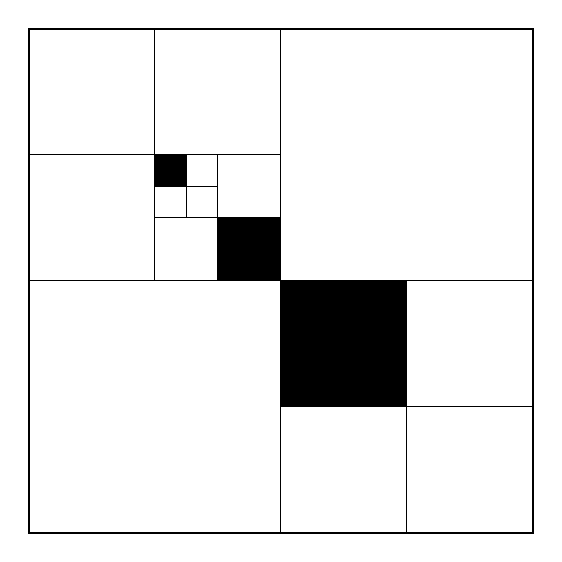
\begin{tikzpicture}[scale=0.8]
            \draw[thick](0, 0)rectangle(8, 8);
            % first division
            \draw(0, 4)--(8, 4);
            \draw(4, 0)--(4, 8);
            % second division
            \draw(0, 6)--(4, 6);
            \draw(2, 4)--(2, 8);
            \draw(4, 2)--(8, 2);
            \draw(6, 0)--(6, 4);
            \fill(4, 2)rectangle(6, 4);
            % third divisions
            \draw(3, 4)--(3, 6);
            \draw(2, 5)--(4, 5);
            \fill(3, 4)rectangle(4, 5);
            % forth divisions
            \draw(2, 5.5)--(3, 5.5);
            \draw(2.5, 5)--(2.5, 6);
            \fill(2, 5.5)rectangle(2.5, 6);
        \end{tikzpicture}
        \captionof{figure}{Hierarchical算法示意图,白块表示稀疏部分}
    \end{center}
\end{theorem}

\begin{theorem}
    {矩阵乘法的Strassen算法}{}
    对矩阵乘法$C=AB$分块得:
    \[
        \begin{bmatrix}
            C_{11}&C_{12}\\
            C_{21}&C_{22}
        \end{bmatrix}=\begin{bmatrix}
            A_{11}&A_{12}\\
            A_{21}&A_{22}
        \end{bmatrix}\begin{bmatrix}
            B_{11}&B_{12}\\
            B_{21}&B_{22}
        \end{bmatrix},
    \]
    定义 
    \begin{subequations}
        \begin{align}
            M_1&=(A_{11}+A_{22})(B_{11}+B_{22}),\\
            M_2&=(A_{21}+A_{22})B_{11},\\
            M_3&=A_{11}(B_{12}-B_{22}),\\
            M_4&=A_{22}(B_{21}-B_{11}),\\
            M_5&=(A_{11}+A_{12})B_{22},\\
            M_6&=(A_{21}-A_{11})(B_{11}+B_{12}),\\
            M_7&=(A_{12}-A_{22})(B_{21}+B_{22}),
        \end{align}
    \end{subequations}
    则
    \begin{subequations}
        \begin{align}
            C_{11}&=M_1+M_4-M_5+M_7,\\
            C_{12}&=M_3+M_5,\\
            C_{21}&=M_2+M_4,\\
            C_{22}&=M_1-M_2+M_3+M_6.
        \end{align}
    \end{subequations}
\end{theorem}

\begin{definition}
    {离散Fourier变换}{discrete Fourier transform}
    式\eqref{eqn:Fourier betaj}中定义了一个线性变换,
    \[
        X_k=\sum_{n=0}^{N-1}x_n\omega^{}
    \]
    变换矩阵为
    \begin{eqnarray}
        F=\begin{bmatrix}
            1&1&1&\cdots&1\\
            1&\omega&\omega^2&\cdots&\omega^{N-1}\\
            1&\omega^2&(\omega^2)^2&\cdots&(\omega^2)^{N-1}\\
            \vdots&\vdots&\vdots&\ddots&\vdots&\\
            1&\omega^{N-1}&(\omega^{N-1})^2&\cdots&(\omega^{N-1})^{N-1}
        \end{bmatrix}
    \end{eqnarray}
    事实上$F$上只有$n$个不同的元素。
\end{definition}
